
\documentclass[main.tex]{subfiles}


\begin{document}

\subsection{\LaTeX}
\label{latex}
\LaTeX je rozšíření jazyku TeX, určenému k sázení dokumentů. TeX je, podobně jako například HTML, značkovací jazyk - formátování výsledného dokumentu je zajištěno množinou značek, které předdefinovaným způsobem ovlivňují vzhled vzniklého dokumentu. Svou filozofií, určení k vytvážení technických a matematických dokumentů, podporuje zápis matematických vzorců, chemických sloučenin i dalších technických specifikací. 
%Je tedy, podobně jako HTML, značkovací jazyk určený pro vytváření pdf dokumentů. Jedná se o sérii maker (předdefinovaných příkazů) k programu TeX, určenému k sázení textu.

\subsubsection{Historie}
TeX byl vytvořen stanfordským profesorem Donaldem Knuthem, počítačovým vědcem. První verzi vydal v roce 1978. Motivací ke vzniku byla nedostatečná kvalita tehdejších sazečských programů na Stanfordské univerzitě a s ní spojená nízká kvalita školních publikací. Na jeho práci navázal Leslie Lamport, jenž vytvořil sadu maker k TeXu, nazývaná \LaTeX. Důvodem byla značná složitost sázení textu v samotném TeXu. \LaTeX svou koncepcí sázení značně zjednodušuje a činí jej dostupnější. 


\subsubsection{WYSIWYG editory}
Jistou alternativou k vytváření dokumentů skrze značkovací jazyky jsou WYSIWYG editory. Poněkud exoticky znějící zkratka pochází z anglického: what you see is what you get. V těchto editorech je upravovaný dokument zobrazován stejně jako výsledný dokument. Typickým příkladem WYSIWIG editorů mohou být programy z kancelářského balíčku Microsoft Office - Word, Excel, Power Point nebo programy LibreOffice.


%\subsubsection{Charakterisika}
%tady umistit nejake priklady značek

\subsubsection{Příklady}
Ukázkový příkladem podpory matematické notace nám poslouží následující zápis matic.

$$
\begin{pmatrix}[cc|cc]
	c & -c & 1 & 0 \\
	c & c & 0 & 1 
\end{pmatrix}
\sim
\begin{pmatrix}[cc|cc]
	1 & -1 & \frac{1}{c} & 0 \\
	1 & 1 & 0 & \frac{1}{c} 
\end{pmatrix}
$$

Tohoto výsledku je docíleno jednoduchou sérií značek: %tady umístíme obrázek
		\begin{figure}[h]
			\centering
			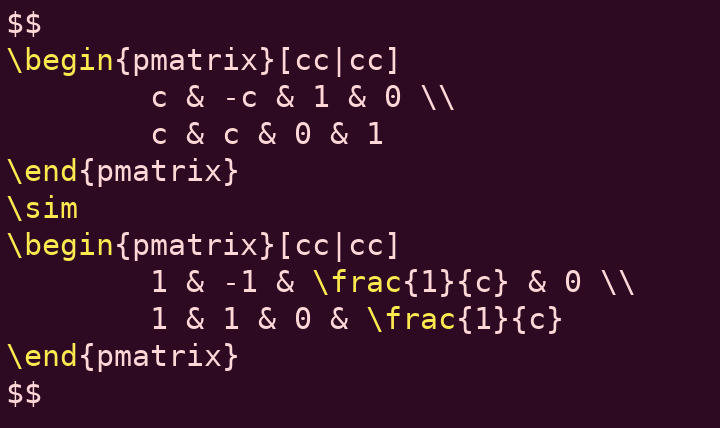
\includegraphics[width=.6\textwidth]{./latex/matrix.png}
			\caption{Vytvoření matice v \LaTeX}
		\end{figure}

\subsubsection{Použití v projektu}
V tomto projektu byl použit \LaTeX spolu mnoha balíčky, jenž slouží k dalšímu rozšíření jazyka. Jedním ze zejímavých balíčků je balíček babel s parametrem czech, který se stará o typografická pravidla jednotlivých jazyků. V tomto případě Češtiny, kdy se sám stará mimo jiné o správné odsazování jednoslabičých spojek, dělení slov a zarovnávání odstavců, které se v Češtině liší od anglického standardu. 

Pro překlad TeXu byl použit konzolový program pdflatex.


\end{document}
